\section{Secure Channels}

\paragraph{Properties:} secure = authentic and confidential, synchronous vs. asynchronous, tunnel vs. transport

\paragraph{Security at different OSI layers:}

\textbf{Application layer:} (Implemented in end-hosts, Email sec.)
\begin{itemize}
\item[+] Extend appl. without involving OS, appl. can understand data and provide appropriate security
\item[-] Security has to be designed separately for each appl.
\end{itemize}

\textbf{Transport layer} (Implemented in end-hosts, TLS, SSL, SSH)
\begin{itemize}
\item[+] Can be added to existing appl., more portable and easier to configure than network layer security
\item[-] Protocol specific (TCP not UDP), appl. must be TLS aware
\end{itemize}

\textbf{Internet layer:} (Secure Traffic over multiple links, IPSec, OpenVPN)
\begin{itemize}
\item[+] Seamless security to Application and Transport Layer, integrated in IPv6 (available for IPv4)
\item[-] Complex configuration on multi-user machines, Tunnel mode encrypts only part of route, depends on policy
\end{itemize}

\textbf{Link layer:} (Secure all traffic over specific link, WPA2 in HW)
\begin{itemize}
\item[+] Speed, seamless security to layers above
\item[-] Every link secured separately, trust in link operator
\end{itemize}

\subsection{VPN}

\paragraph{Goal:}  Securely interconnect networks or machines over an existing network (ex.: link branch offices via insecure WANs) 
\begin{itemize}
\item uses public network as transport layer
\item uses cryptography to provide protection (symmetric with secret key, asymmetric with public and private key, encrypt payload only/and header) 
\item provides confidentiality and authenticity
\item IP in IP encaps. (remote LANs appear adjacent)
\end{itemize}

\paragraph{Operation modes:} ESP = Encapsulating Security Payload, AH = Authentication header \\
\emph{Tunnel mode:} encapsulate entire encrypted IP packet
no routers along the way need to examine
the inner IP header. \\ 
\emph{Transport:} encrypt payload only

\begin{tabular}{p{0.2\linewidth}p{0.7\linewidth}}
\textbf{AH+ESP} & The payload is encrypted by ESP and the payload and parts of the outer IP header are authenticated by AH \\
\hline
\textbf{ESP+Auth} & Encryption and ESP's data origin authentication are applied to the payload only \\
\end{tabular}

AH+ESP has two benefits over ESP+Auth since it allows for IP header auth. and it allows for auth. and encryption to be handled by two different entities (e.g., auth. on end-host, encryption on firewall)

\paragraph{IPSec Security Association (SA):} used to lookup security algorithms/parameters to apply
to a received IPSec datagram; separate for ESP and AH, unidirectional; need two SAs for a bidirectional channel, SA setup: manual or with IKE (Internet Key Exchange)

SA is uniquely defined by a triple of \emph{Security Parameter Index (SPI):} 32 bit num. placed in AH or ESP datagrams, \emph{IP dest. addr.:} address of device for whom SA is established and \emph{Security Protocol Identifier:} AH or EH. Specifies whether SA for AH or ESP

\textbf{Attacks on VPN}

\begin{tabular}{p{0.15\linewidth}p{0.4\linewidth}p{0.3\linewidth}}
Type & Attack & Remedy \\
\hline
\hline
Passive & Eavesdropping & Sender encrypts every packet \\
\hline
Active & MitM, add, modify, delete data packets & Sender signs every packet with a secure hash (provides integrity and authenticity)\\
\hline
Replay (active) & Reproduce and inject packets (captured earlier); example: replay ``pay 1\$'' 100 times to harm victim & Embed UID or timestamp in every packet before signing
\end{tabular}

Both SSL and TLS support above protection. When using SSL, authentication has to be explicitly turned on before the initial key exchange (client-server-auth.).

\paragraph{Message Authentication} 
\begin{itemize}
\item used to check source authenticity, message not modified (error code), message timing (timestamp), sequence (number)
\item only $A$ and $B$ share a key $K$ (conventional encryption) 
\item at $A$ append MAC to message $M$: $MAC = f(K_{AB}, M)$. Full packet: $M + MAC$
\item compare MACs at $B$
\end{itemize}

\paragraph{HMAC} MAC using hash functions (MD5, SHA, ....) \\ \emph{Advantages:} fast, source code free and available, no patents or export restrictions
\dm{
\text{HMAC}(K, M) = f_h(K' \text{ XOR } opad + f_{h}(K' \text{ XOR } ipad + M))
}
$K'$ = key padded with 0x0's, $opad$ = 0x5C, ipad = 0x36 (all padded to length 64 bytes)

\paragraph{VPN Security:} Encryption must be combined with authentication (HMAC), randomized Initialization Vectors (IVs), replay protection

\subsection{TLS}

Transport Layer Security. Provides communications privacy, prevents eavesdropping, tampering, or message forgery by: authentication (using public key certificates), encryption, data integrity.

\pgra{Goal:} perform secure e-commerce (banking, shopping, web login e.g. gmail)

\pgra{Diffie-Hellman key exchange:} establishes a shared secret that can be used for secret communications by exchanging data over an insecure channel. The simplest,  implementation of the protocol uses the multiplicative group of integers modulo $p$, where $p$ is prime and $g$ is primitive root mod $p$.

\begin{tabular}{ccc|c}
\multicolumn{1}{c}{\textbf{Alice:} secret $a$} & &  \multicolumn{1}{c}{\textbf{Bob:} secret $b$} & \\
Calculates & Sends & Calculates & Public \\
\hline
\hline
 & $p$, $g\to$ & & $p$, $g$ \\
$g^a$ mod $p$ = A & $A\to$ & & $p$, $g$, $A$ \\
 & $\leftarrow B$ &$g^b$ mod $p$ = B & $p$, $g$, $A$, $B$ \\
 $B^a$ mod $p = \mathbf{s}$ & & $A^b$ mod $p = \mathbf{s}$ & $p$, $g$, $A$, $B$ \\
\end{tabular}

where $\mathbf{s}$ is the established secret $\Rightarrow$ color-mixing example.

\pgra{Man-in-the-middle on DH:} DH is susceptible to a MitM attack when certificates aren't used. Attacker situates themselves between A and B and impersonates A to B and B to A. Certs can be used to prevent DH MitM.

\textbf{SSL/TLS Protocol}\\
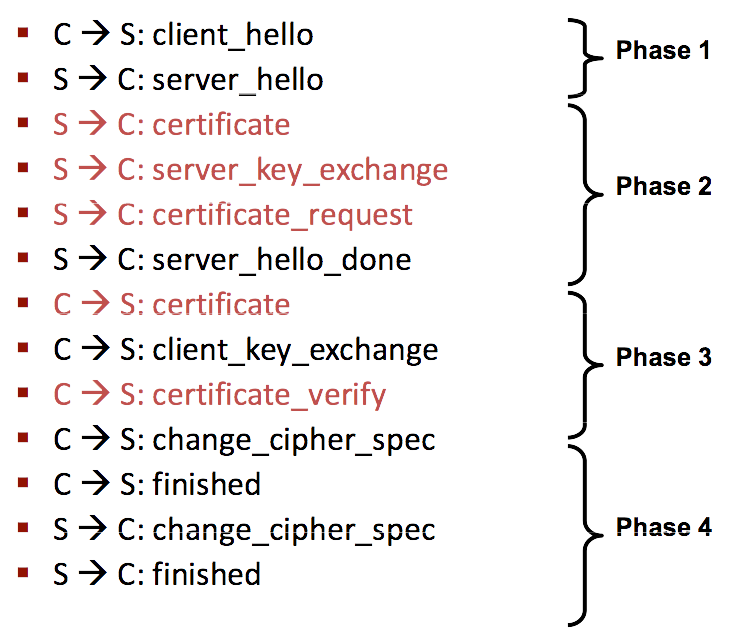
\includegraphics[width=7cm]{images/SSLProtocol}

\pgra{Phase 1:} Establish security capabilities.\\
{client,server}\_hello\_message containing: highest supported version, random = 32bit timestamp | 28 bytes rand, session ID, client\_hello: supported cihper suite in decreasing order of preference, server\_hello: chosen cipher.

\textbf{Potential attack:} "dumbing down" - MitM removes strong ciphers from client\_hello, prevention: HMAC in Phase 4

\pgra{Cipher specs}
\bitem{
\item Cipher algorithm (RC4, RC2, DES, 3DES, DES40, IDEA, AES, Camellia)
\item MAC Algorithm (MD5, SHA-1, SHA-256)
\item Cipher type (stream or block)
\item Is exportable (true/false)
\item Hash size (0 or 16 for MD5, 20 for SHA-1, 32 for SHA-256)
}

Minimum no. of bits for symm. crypto: 80, 128 is better - should be secure until 2040.

\pgra{Key Exchange Mechanisms Analysis Metrics:}
\bitem{
\item Secure against passive attacker?
\item Secure against MitM attacker?
\item Perfect Forward Secrecy: Compromise of lont-term private key does not reveal session key
\item Contributory key agreement: Both parties contribute to session key, no party can fully determine session key
}

\textbf{RSA Key Exchange (Case 1)}
\bitem{
\item Server has RSA key than can encrypt
\item Client creates pre-master secret session key and sends it to server encrypted with server's public RSA key $K_S$
\item Phase 2\&3 Messages
\bitem{
	\item S $\rightarrow$ C: Server cert $\left\{\text{URL}, K_S\right\}_{K_{CA}^{-1}}$
	\item S $\rightarrow$ C: server\_hello\_done
	\item C $\rightarrow$ S: client\_key\_exchange: $\left\{K\right\}_{K_S}$
	}
\item Metrics: Secure against passive and active attacks, no PFS, no contributory key agreement
}

\pgra{RSA Key Exchange (Case 2)}
\bitem{
\item Server has RSA key that can sign but not encrypt (trick: generate temporary public/private keypair $K'_S/K'^{-1}_{S}$)
\item Phase 2\&3 messages:
\bitem{
	\item S $\rightarrow$ C: Server cert $\left\{ \text{URL}, K_S\right\}_{K_{CA}^{-1}}$
	\item S $\rightarrow$ C: Server key exchange $\left\{\text{URL}, K'_S\right\}_{K_{S}^{-1}}$
	\item S $\rightarrow$ C: server\_hello\_done
	\item C $\rightarrow$ S: client\_key\_exchange $\left\{K\right\}_{K'_S}$
	}
\item Metrics: Secure against passive and active attacks, PFS, no contributory key agreement
}

\pgra{Fixed DH Key Exchange}
\bitem{
\item Server has DH certificate
\item Phase 2\&3 messages
\bitem{
	\item S $\rightarrow$ C: Server cert $\left\{ \text{URL}, g^S\mod p \right\}_{K_{CA}^{-1}}$
	\item S $\rightarrow$ C: server\_hello\_done
	\item C $\rightarrow$ S: client\_key\_exchange $g^C \mod p$
	}
\item Metrics: Secure against passive and active attacks, no PFS, contributory key agreement
}

\pgra{Ephemeral DH Key Exchange}
\bitem{
\item Server has certificate for RSA signing key
\item Phase 2\&3 messages:
\bitem{
	\item S $\rightarrow$ C: Server cert $\left\{\text{URL}, K_S\right\}_{K_{CA}^{-1}}$
	\item S $\rightarrow$ C: Server key exchange: $g, p, g^S, \left\{g^s\right\}_{K_S^{-1}}$
	\item S $\rightarrow$ C: server\_hello\_done
	\item C $\rightarrow$ S: client\_key\_exchange: $g^C \mod p$
}
\item Metrics: Secure against passive and active attacks, PFS, contributory key agreement
}

\pgra{Anonymous DH Key Exchange}
\bitem{
\item No certificates
\item Phase 2\&3 messages:
\bitem{
	\item S $\rightarrow$ C: Server key exchange: $g,p, g^S \mod p$
	\item S $\rightarrow$ C: server\_hello\_done
	\item C $\rightarrow$ S: client\_key\_exchange: $g^C \mod p$
	}
\item Metrics: Secure against passive attacks, not secure against MitM, PFS, Contributory key agreement
}

\pgra{SSL Phase 2}
\bitem{
\item After Phase 1, both parties know which key exchange mechanism and cipher to use
\item Phase 2: server authentication and key exchange
}

\pgra{SSL Phase 3}
\bitem{
\item After Phase 2, client has required values to generate session key
\item Phase 3: client authentication and key exchange
}
\pgra{SSL Phase 4}
\bitem{
\item After Phase 3, client and server share master secret and authenticate each other
\item Phase 4 contains HMAC of master\_secret and handshake messages
}

\pgra{Cryptographic computations:} Master secret computed from pre-master secret, client random and server random. Master secret is then used with a PRNG function to produce a pseudorandom bitstream.

\pgra{Studies on SSL indicators}
\bitem{
\item $\approx 50\%$ cannot identify connection as secure or not
\item $85\%$ know about lock icon, $65\%$ know it should be part of browser (not in page)
\item $65\%$ never noticed https prefix
\item $23\%$ rely solely on webpage content to determine legitimacy
\item $9\%$ look at certificate
}

\pgra{Certificate Revocation:} mechanism to invalidate certificates (e.g. after private key exposed, employee leaves corporation, expiration time too far in future). CAs periodically publish Certificate Revocation Lists (CRLs), delta CRLs only contain changes (what if CRL update missed?). General problem with revocation: CAP theorem (Consistency, Availability, tolerance to Partition) - impossible to acheive all 3.

\pgra{OCSP:} Online Certificate Status Protocol to verify cert. status, ensure cert. valid and not revoked (cert. contains OCSP responder). Issues: falsified cert. would use own server as OCSP, browser doesn't want to fail should OCSP server not respond/be blocked.

\pgra{Compelled Certificates:} Governments allowed to perform active MitM attacks. Cert. issued with signing rights, used in a MitM device to create new cert. for pages on-the-fly. Dangers: devices with compelled certs. being stolen.

\pgra{SSL/TLS PKI Statistics:} 1482 certs. trusted by Microsoft/Mozilla, 1167 distinct ``issuer'' strings, 651 organisations. 16.2M IPs listening on port 443, 11.3M start SSL handshake, 4.3M used valid cert. chains, 1.5M distinct valid leaves.

\pgra{Assumptions for Secure SSL:}
\bitem{
\item CA: (no CA root key compromised, no employee of any CA can issue bogus cert. All CAs thoroughly verify owner of domain)
\item Crypto: (all crypto algorithms are ``secure'')
\item Browser: (all root certs. in browser correct, browser doesn't contain remotely explotable vulnerabilities, malicous sites cannot overwrite lock/https, no unicode/homograph vulnerability)
\item User: (checks for https and closed lock, cannot be tricked into bogus URL, does not accept bogus cert., does not ignore cert. warnings)
}
If any of these does not hold, SSL not secure!

\pgra{Handshake Protocol:} executed before the appl. protocol transmits or receives any data, negotiation of encryption MAC and compression algo. and cryptographic keys. After TLS handshake procedure finished transmitted appl. data is encrypted and server and optionally client are authenticated. (Client encrypts secret with public key, server decrypts with private key $\to$ master secret)

\pgra{Server authentication:} done via X.509 Server Public Key Certificates. Trusted Certificate Authority (CA) signs cert. with private key, client browsers get the CA's public key.\\
Upon TLS secured site visit: browser checks\\ {\tt hash(certificate) == decrypt(public key, signature)}.\\
Server needs (a) the CA-signed TLS certificate (b) its corresponding private key.

\pgra{Key size(s):} SSL and TLS support keys 40-bit RSA keys, 56-bit DES keys (both deemed too short and thus insecure) and 128-bit (or higher) keys (secure).

\pgra{Purpose of a certificate:} Secure container for a public key,
Issued by a trusted third party,
Issued to a subject (owner),
Valid for a limited time,
Usable for a limited purpose,
Information Fields

\pgra{Content of a X.509 certificate:} Unique Identifier, Issuing CA, Validity, Owner, Public key, Purpose, Name alternatives, Extended purpose, KeyID of Issuing CA, Revocation Info, Online verification, CA signature

\textit{The CA flag in the certificate shows whether it is a signing certificate or an end-user certificate.}

\pgra{Structure of a PKI:} From (1): highest trust to (4): end-user certificates
\begin{enumerate}
\item Root CA: Self signed, Offline, highest trust
\item Subsidiary CA: Offline/Online, Issues CAs
\item Issuing CA: Online, Issues end-user certificates
\item Certificates: certificates bought for business (e.g. securing e-commerce, etc.)
\end{enumerate}

\pgra{Technical issues with X.509 certificates:} 
\bitem{
\item Compromise of private keys
\item Inadequate algorithms/key sizes
\item Incomplete verification (rfc 5280): Certificate Validation (Integrity, Validity, etc.),
Path validation (20 Pages in rfc 5280),
Revocation status verification
}

\pgra{Root CA:} a CA with a self-signed certificate (there's 'no one above it'). To trust a certificate signed by this CA, it must necessarily be in the ``trusted CA list'' of every browser

\subsection{SSH}

\paragraph{Definition:} standard for remote logins and encrypted file transfer, provides secure command shell, secure file transfer, data tunneling, fully negotiable. 
\\Three protocols: \textbf{SSH-TRANS}, \textbf{SSH-AUTH}, \textbf{SSH-CONN}

\paragraph{SSH-TRANS:} fundamental SSH building block, runs over TCP. Provides: algorithm negotiation, key exchange (Diffie-Hellman) (repeated every h/Gb), Session ID, server authentication, encryption, integrity, data compression. All parameters are negotiable (security implications).

\paragraph{SSH-AUTH:} used over SSH-TRANS to authenticate client \\
Provides: framework for authentication mechanisms\\
Authentication request is client driven, contains: username U, method name M and method specific data D, Service name S (facility to which client requests access)
\textbf{Authentication Methods}
\begin{itemize}
\item Public-key user authentication (test if use has access, perform authentication)
\item Password authentication (SSH-CONN encrypts) 
\item Host based authentication\\
\quad User authentication: responsibility with client host\\
\quad Host authentication: trust relationships between hosts, server verifies host identity
\end{itemize}

\paragraph{SSH-CONN:} used after SSH-AUTH to provide richer services over SSH-TRANS conn. Provides: multiplexing multiple streams (channels), port forwarding, compression handling\\
\emph{Port forwarding:} Encrypt/decrypt traffic for other TCP/IP applications, securing otherwise insecure protocols. Local/\\remote forwarding: forward local port to remote server port, forward remote server port to local host port (i.e. if port 80 is blocked by firewall)

\paragraph{Attacks SSH can counter}
\begin{itemize}
\item Eavesdropping $\to$ encryption in SSH-TRANS
\item Name service and IP spoofing $\to$ crypt. verified server ID (SSH-TRANS) 
\item Connection-hijacking $\to$ not preventable on TCP-level, integrity checking (MACs checked by SSH-TRANS)
\item Man-in-the-middle $\to$ server authentication: public key + host based
\end{itemize}

\paragraph{Attacks SSH can NOT counter}
\begin{itemize}
\item Password cracking $\to$ rather social problem
\item IP and TCP attacks, SSH operates on TCP (DoS: SYN flood, TCP RST, ICMP bogus, TCP desynch.)
\item traffic analysis (possible to watch data amount, src/dest, timing)
\end{itemize}

\section{WebApp Security}
\paragraph{Top 5 Application Security Flaws:} 1. Injection flaws, such as SQL, OS, and LDAP injection, 2. Cross Site Scripting (XSS)
3. Broken Authentication and Session Management
4. Insecure Direct Object Reference
5. Cross Site Request Forgery (CSRF)

\paragraph{Threat Vectors - Web Application:} Abuse client (XSS, Phishing), abuse link (session hijacking), abuse application (XSS), abuse database (SQL injection). \\
Direct access to application by definition (HTTP: 80, HTTPS: 443). Even through secure encrypted tunnel.

\subsection{Session Management}

\paragraph{HTML - Stateless Protocol} The server does not know which clients connects again. Any meaningful application needs state info. We have to implement session state ourselves.

\paragraph{Adding State to HTTP} Server creates a SessionID upon first contact. Client stores SessionID locally. Client submits SessionID with every request to server. Server identifies client based on SessionID and stored session state.

\paragraph{Session State and Security}
SessionID is a primary target for an attacker. Crucial processes: Generation, Transport, Destruction and Revocation of SessionID. Session management is crucial to the secure operation of an application.


\paragraph{Session - Generation}
Strength: The SessionID must not be predictive. Randomness: strong method of generating ID's, don't use linear algorithms based on time, date, processid, or client IP

\paragraph{Session - Revocation}
Session timeout, client (logout) and server (no activity, misuse) able to revoke, expiry time set to minimum

\paragraph{Session - Transport} 
Three ways to transport the session ID: HTTP GET, HTTP POST, Cookies

\paragraph{Cookies:} A piece of information stored in the browser. Cookies are restricted to domain, path and are given an expiration date. The server sets a cookie, the browser submits cookies back. Cookies can be restricted to HTTPS connections only. Cookie information submitted in request/response header. (Set-Cookie: 6B=DB98, Cookie: 6B=DB98)

\paragraph{Attacks on session ID}
\begin{itemize}
\item Observation: Sniffing Attack: HTTP unencrypted $\to$ use HTTPS \emph{throughout} the session!
\item Brute Force Attack:\\ \quad Passwords: the SessionID has to be random \\ \quad Username: must not be predictable (brute force, DoS)
\end{itemize}

\begin{tabular}{p{0.15\linewidth}p{0.3\linewidth}p{0.4\linewidth}}
Type & Advantage & Disadvantage \\
\hline
\hline
HTTP GET & Easy to implement, compatibility (no cookies needed)  &  Reviewable in browser history, URL information is logged on several devices (firewalls, server, proxy), trivial exercise to manipulate SessionID, when the client clicks a link to new website HTTP REFERER reveals session information \\
\hline
HTTP POST & Not as obvious as URL embedded SessionIDs, allows client to safely store/transmit URL info, compatibility & Hidden fields not really hidden, easy to manipulate, more complex webpage creation processes necessary, prone to coding error \\
\hline
Cookies & More options available to control SessionID's, session information unlikely to be recorded on intermediate devices, built in ability to restrict cookie-submission to HTTPS connections only & Persistent cookies exist as files on the clients file-system, may be stolen, any request to the domain will provide the cookie, if the cookie-path matches, users may disable cookies \\
\end{tabular}

\subsection{SQL Injection}

\paragraph{Code injection:} refers to attacks which insert code that is afterwards interpreted by a process. \emph{Examples:} Command/Shell Injection (target: OS), XSS (Browser), SQL Injection (Database). Occurs when:
\begin{itemize}
\item Data enters the application from an untrusted source
\item The data is part of a string that is executed as a command by the application
\item The executed commands elevates privileges or capabilities the attacker normally wouldn't have
\end{itemize}

\paragraph{SQL - Structured Query Language} SQL is a special-purpose programming language designed for managing data in relational database management systems (RDBMS). Includes \emph{view, insert, query, update} and \emph{delete} operations.

\begin{tabular}{p{0.35\linewidth}p{0.6\linewidth}}
Command & Description \\
\hline
\hline
SELECT FROM & Extract data from a specific table. One entry can be retrieved with WHERE statement \\
INSERT INTO & Insert data into a specific table \\
DELETE FROM & Delete data from a specific table\\
UPDATE & Update data in the table to a new value \\
CREATE & Create a new table\\
DROP & Delete the entire table (!) \\
ALTER & Change a table \\
UNION & Retrieve data from more than one table (number of columns must match) \\
\end{tabular}

\paragraph{SQL Code Injection:} insertion of a SQL query via the input data from the client to the application. A successful SQL injection can
\begin{itemize}
\item read sensitive data from the database
\item modify database data (insert / update / delete)
\item execute administration operations on the database
(such as shutdown the DBMS)
\item recover the content of a given file present on the DBMS file
system
\item issue commands to the operating system
\end{itemize}
\emph{SQL injection attacks result from flaws in the WebApp, not from flaws in the database or webserver!}

\paragraph{Example:} Select user id and login upon login of user \emph{xyz}: \\
\\
{\tt SELECT userid, login FROM users WHERE login='xyz'}\\ {\tt AND pwd='swordfish'} \\
\\
Can be exploited using {\tt ' OR ''='} as login and/or {\tt ' OR ''=''} as password:\\
\\
{\tt SELECT userid, login FROM users WHERE login=} \\ {\tt '' OR ''='' AND pwd='' OR ''=''} \\
\\
Above statement will always return TRUE and return all records in table {\tt users}. The attacker is authenticated as the first user in the table.

\textbf{Other attacks:} {\tt UNION} to read (unauthorized) from other tables, {\tt DROP} table to delete user/customer data, advanced/\\blindfolded SQL injection, combination of {\tt ;} (statement termination) and {\tt --} (comment) to run any SQL command.

\paragraph{SQL injection defense} The following will not circumvent SQL injection attacks:
\begin{itemize}
\item VPN, SSL and Firewalls (the attack occurs when using a \emph{legitimate} channel)
\item client-side input validation (can be easily circumvented by an attacker)
\end{itemize}
Instead, do the following:
\begin{itemize}
\item[+] \textbf{constrain and sanitize all client data}
\\ \quad PHP: {\tt mysql\_real\_escape\_string} function
\item[+] avoid disclosing detailed error information
\item[+] do not use client data directly in SQL queries (use prepared statements, parametrized queries)
\item[+] run the database process with reduced privileges
\item[+] Check all entry points: (a) fields in web forms, (b) script parameters in URL query strings, (c) values stored in cookies or hidden fields
\end{itemize}

\pgra{Prepared statements:} A prepared statement or a parametrized statement is used to execute the same statement repeatedly with high efficiency. The basic workflow consists of the following steps:

\begin{enumerate}
\item Prepare stage: a statement template is sent to the database server. The server performs a syntax check and initializes server internal resources for later use.
\item Bind and execute: the client binds parameter values and sends them to the server. The server creates a statement from the statement template and the bound values to execute it using the previously created internal resources.
\item Repeated execution: the statement is not parsed again and the statement template is not transferred to the server again.
\end{enumerate}

\textit{Injection defense:} Bound variables will be escaped automatically by the server. The server inserts the escaped values at the appropriate places into the statement template before execution. A hint must be provided to the server for the type of bound variable, to create an appropriate conversion.

\paragraph{Other attack strategies} Fuzzing (insert {\tt ' " ) \# || + >} into every entry field), delay query, order by $n$, get metadata: {\tt sysobjects, syscolumns} \\
IDS evasion: try all the flavors of {\tt OR 1=1}, insert whitespaces, comments in between statements, wildcards, concatenation, etc.
